\section{Introduction}
\label{sec:intro}

\begin{figure}[t]
  \centering
  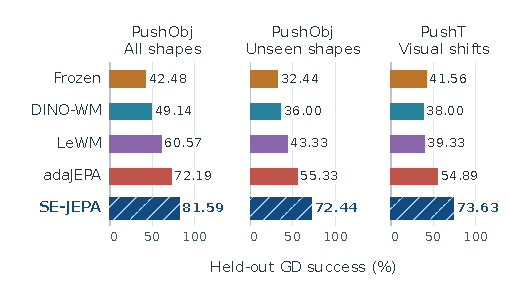
\includegraphics[width=\linewidth]{teaser_bars.pdf}
  \caption{\textbf{Deployment experience improves held-out planning.} Held-out success with CEM planning on PushObj shapes, the three shapes unseen during pretraining, and six PushT visual shifts.}
  \label{fig:teaser_bars}
\end{figure}

World models let an agent try actions in imagination before committing to them. Latent world models make this practical for visual control: they predict how an encoded scene evolves under candidate actions, and a model-predictive controller (MPC) searches for the action sequence whose predicted outcome matches an image goal~\cite{zhou2024dinowm,wang2026straightening,maes2026lewm}. Planning is only as good as these predictions. When a deployed agent meets an object shape or a visual appearance it was not trained on, prediction errors turn directly into planning failures.

Test-time adaptation offers a remedy. AdaJEPA~\cite{wang2026adajepa} treats every executed action as free supervision: the observed transition corrects the predictor before the next replan. This closes a second feedback loop around MPC and recovers much of the lost performance within an episode. The correction, however, is discarded when the episode ends. An agent that pushes the same unfamiliar object a hundred times relearns its dynamics a hundred times.

We ask whether a world model can instead \emph{remember} what it learns during deployment. The key is to turn local corrections into reusable predictions. A fast update fits a short trajectory around one start and goal; across episodes, these updates point in nearly orthogonal directions. Directly retaining them does not reliably produce a predictor that serves the full stream. On a matched stream, full accumulation lowers success from 62\% to 48\% (Sec.~\ref{sec:diagnosis}). What should persist is the experience behind an update, not the update itself.

\begin{figure*}[t]
  \centering
  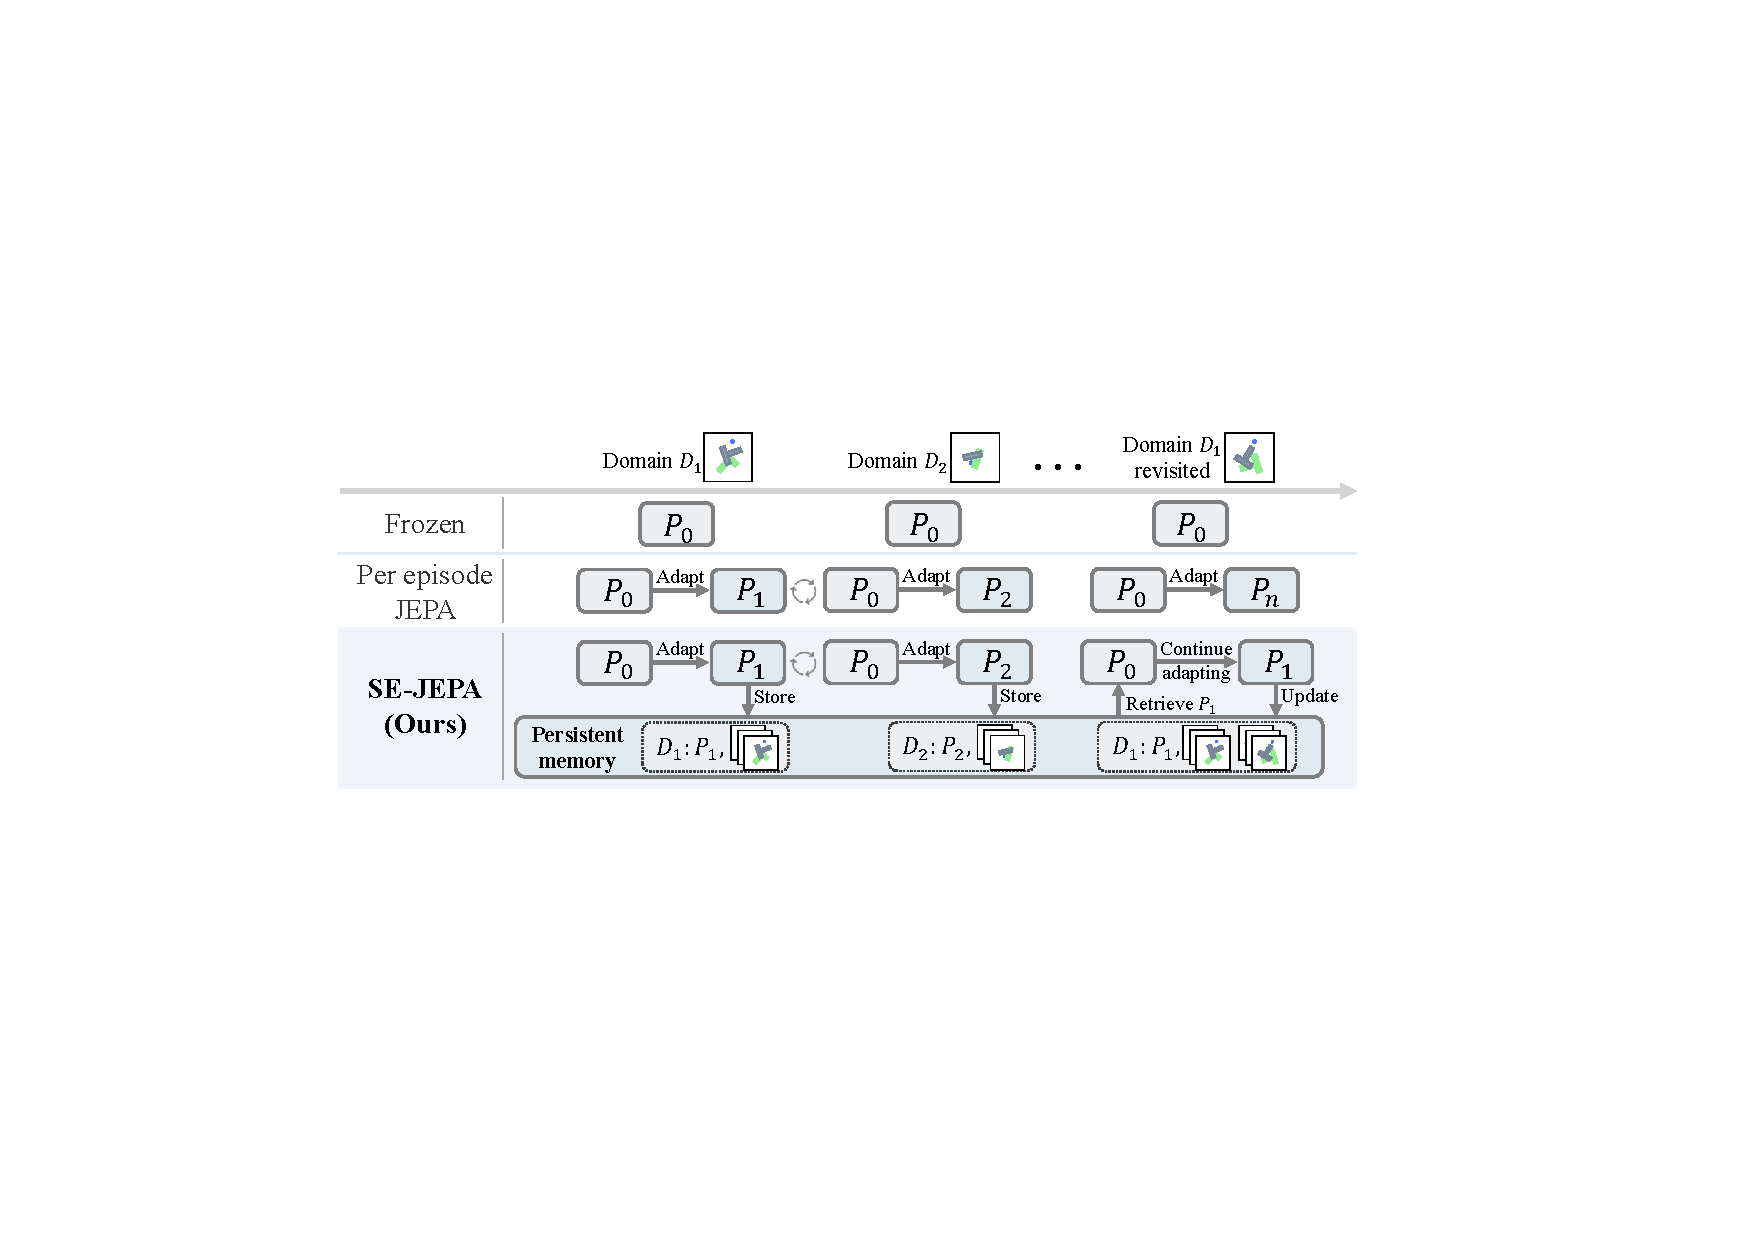
\includegraphics[width=\textwidth]{comparison.pdf}
  \caption{\textbf{From episodic adaptation to self-evolution.} A frozen world model plans every episode with the same predictor. Single-episode adaptation repairs the predictor during an episode and resets it afterwards. \ours consolidates experience into slow learners by replay and retrieves them when a shift recurs, so experience from earlier episodes can improve later planning. Domain names are for illustration; the method receives no labels.}
  \label{fig:comparison}
\end{figure*}

We introduce \ours, a self-evolving latent world model built on complementary learning systems~\cite{mcclelland1995cls}. A fast system adapts within the episode exactly as AdaJEPA does. A slow system stores the episode's transitions in the fixed latent space of the pretrained encoder and consolidates them into slow predictors by replay, one per domain that the model discovers on its own. Prediction errors and fast-update fingerprints organize this memory without domain supervision. The error of the pretrained predictor tells \ours whether an episode contains anything new. The direction of the fast update tells it which domain the experience belongs to. The error of a slow predictor on episodes it has not yet trained on tells it when that predictor can be trusted for planning. The pretrained model is never modified, so the agent can always fall back to it.

This design connects continual learning directly to visual control. With both gradient descent (GD) and the cross-entropy method (CEM), \ours improves held-out planning on PushObj shapes and PushT visual conditions (Fig.~\ref{fig:teaser_bars}). These gains use task-trained ResNet backbones; slow consolidation also improves DINO-WM on rope and granular manipulation, extending persistent learning to a different visual representation and deformable dynamics. With CEM it reaches 79.1\% success on held-out shapes and 69.9\% on unseen shapes, against 70.4\% and 54.4\% for AdaJEPA; under recoloring of the object or goal its gains exceed 27 points. Its online success improves over deployment rounds, and on deformable objects it reduces Chamfer distance by 49\% (rope) and 27\% (granular) relative to DINO-WM.

Our contributions are:
\begin{itemize}
  \setlength{\itemsep}{1pt}
  \item We identify experience replay as the bridge from episodic adaptation to persistent latent planning, motivated by a matched-stream diagnosis of weight accumulation.
  \item We propose \ours, which turns transient adaptation into lasting predictive knowledge through replay consolidation, self-discovered domains, and validation before retrieval, using prediction errors and fast-update fingerprints.
  \item We demonstrate persistent learning with task-trained ResNet and DINO-WM backbones across rigid and deformable manipulation, with higher held-out success and fewer interactions under both GD and CEM on rigid-object tasks.
\end{itemize}

\begin{figure*}[t]
  \centering
  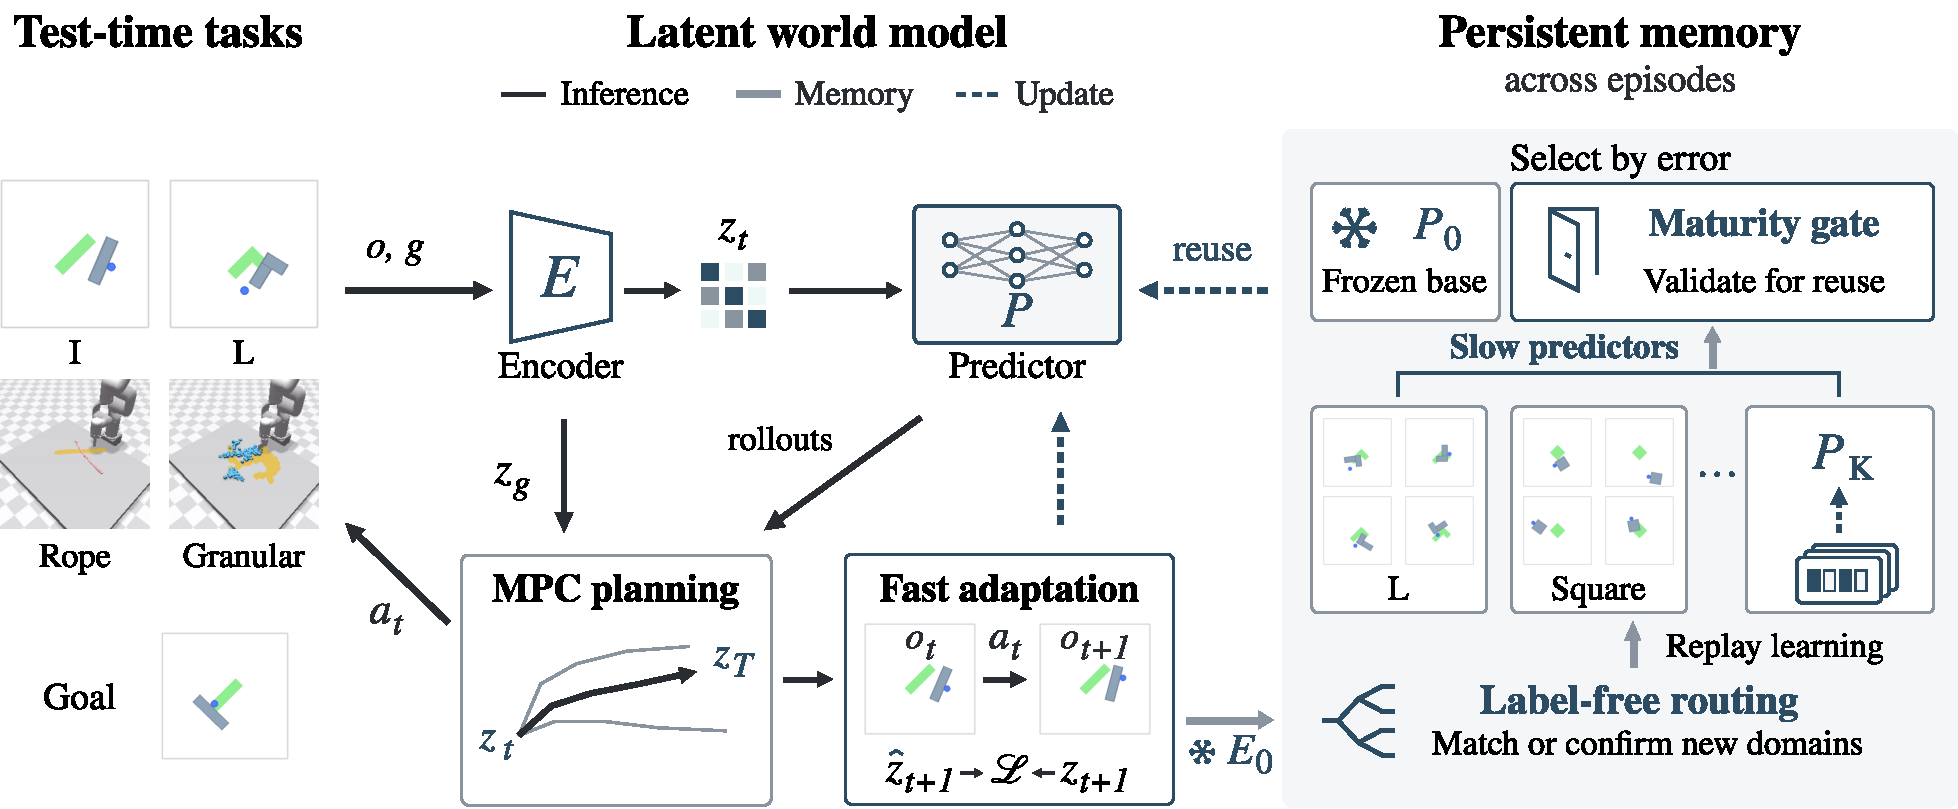
\includegraphics[width=\textwidth]{architecture.pdf}
  \caption{\textbf{\ours architecture.} The fast loop plans in latent space and adapts the predictor from observed transitions. At the end of an episode, the slow system re-encodes the trajectory with the frozen encoder, assigns unfamiliar experience to a self-discovered domain, and trains that domain's slow predictor by replay. Predictors that pass the maturity gate compete with the frozen base at the start of the next episode. Fast parameters reset at every episode; slow predictors and replay persist. Shape names illustrate memory contents and are not supervision.}
  \label{fig:architecture}
\end{figure*}
